\documentclass[compress]{beamer}
\usepackage[ngerman]{babel}
\usepackage{graphicx}
\usepackage{subfiles}
\usepackage{listings}

\graphicspath{{resources/}}

% \setbeameroption{show notes}

\usetheme[noflama]{custom}

\title{Funktionale \break Programierung}
\subtitle{Nebenläufigkeit \& Parallelisierung}
\author{Jan-Philipp Willem}
\institute{Prof. Dr. Sandro Leuchter\\
  Fakultät für Informatik\\
  Hochschule Mannheim
}
\date{Seminar, WS2016}

\begin{document}

\begin{frame}[noframenumbering,plain]
  \frametitle{Was wird hier gezeigt?}
  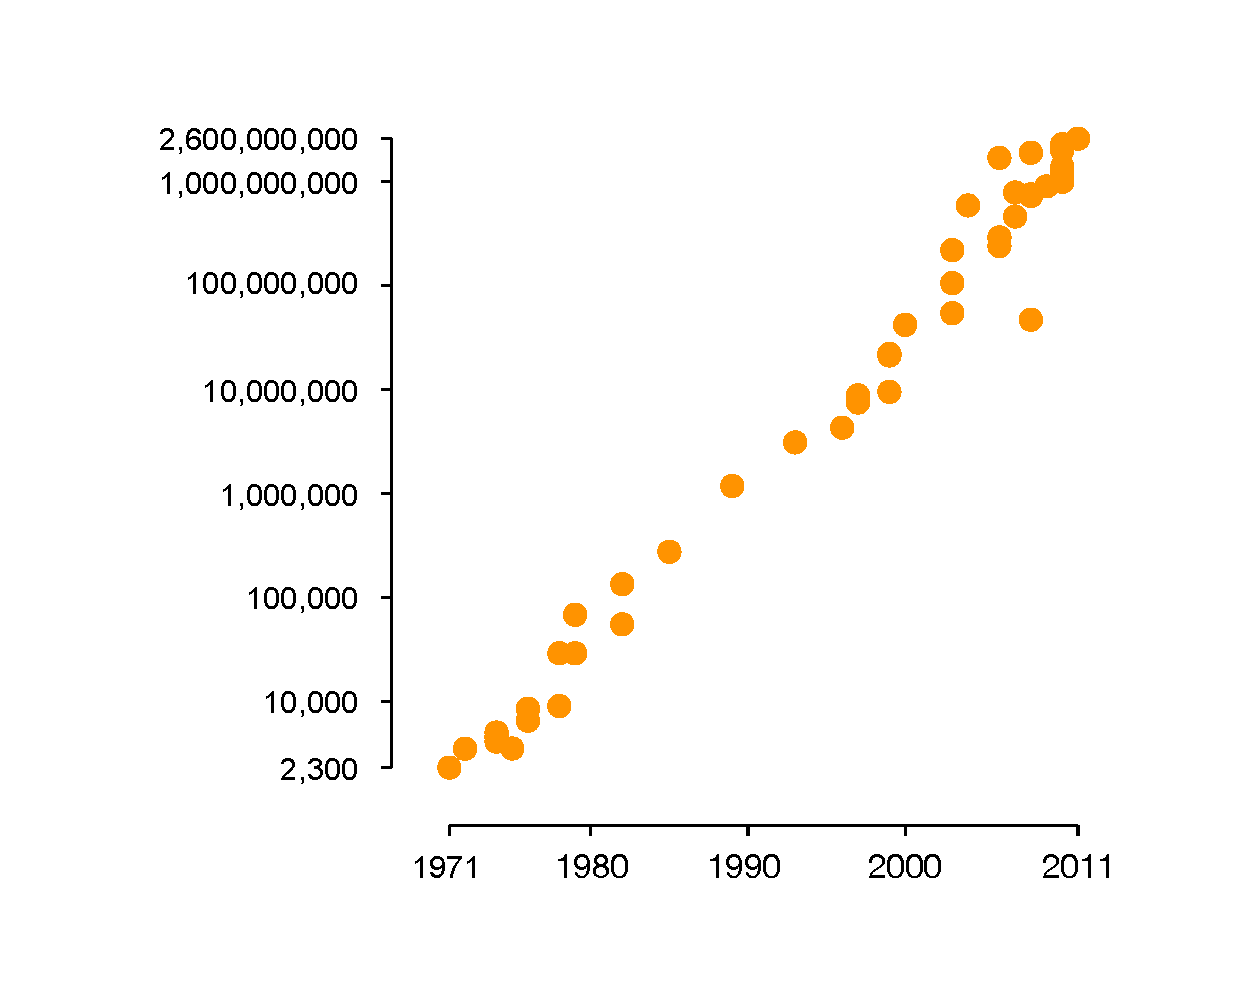
\includegraphics[width=0.9\textwidth]{moores_law.pdf}
\end{frame}

\begin{frame}[noframenumbering,plain]
  \frametitle{Transistor Counts 1971-2011 \& Moore's Law}
  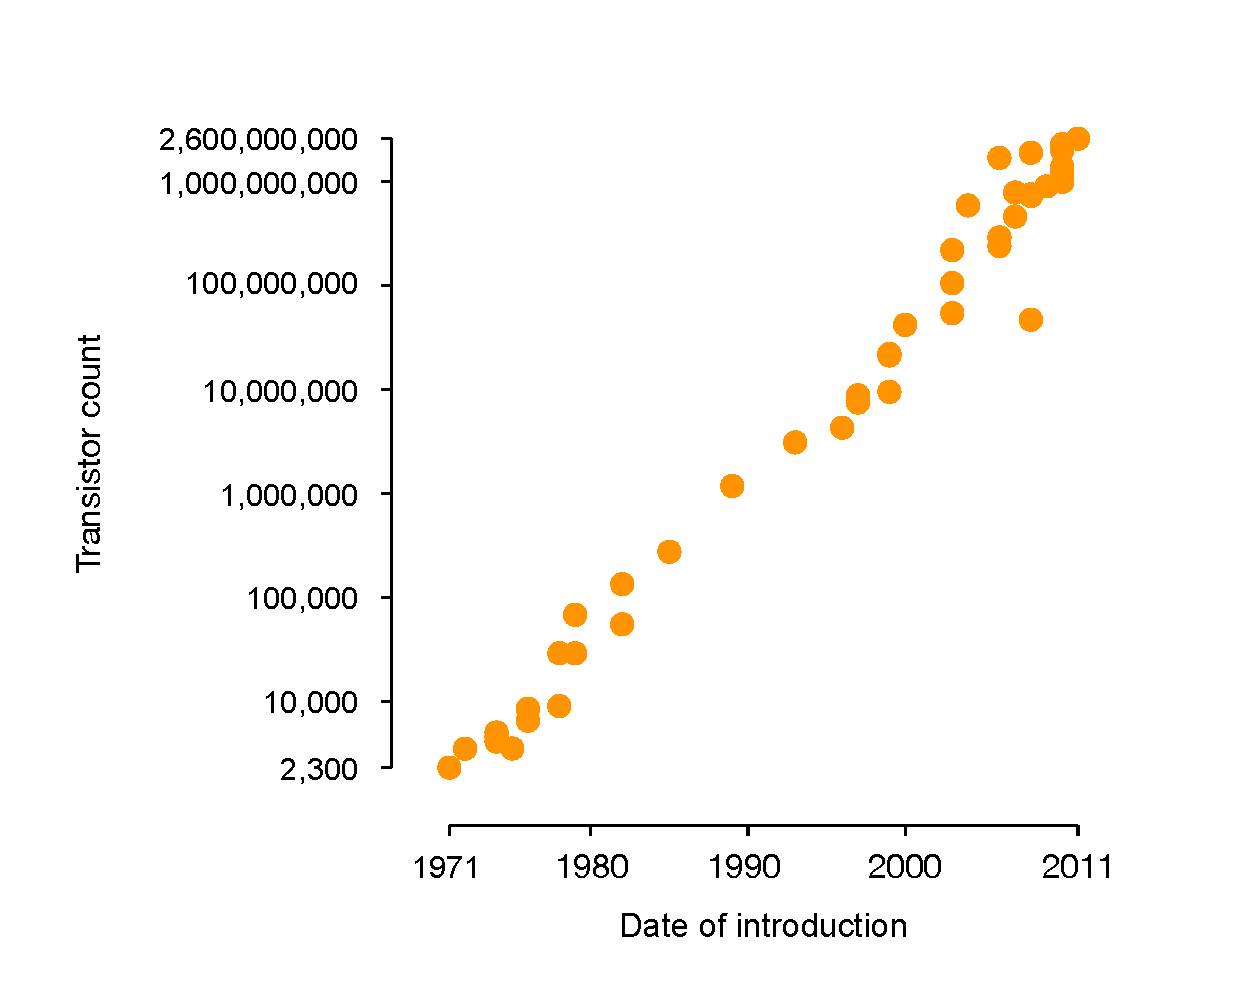
\includegraphics[width=0.9\textwidth]{moores_law_with-labels.pdf}
\end{frame}

\begin{frame}[noframenumbering,plain]{arsTECHNICA UK - 03.01.2017 (1)}
  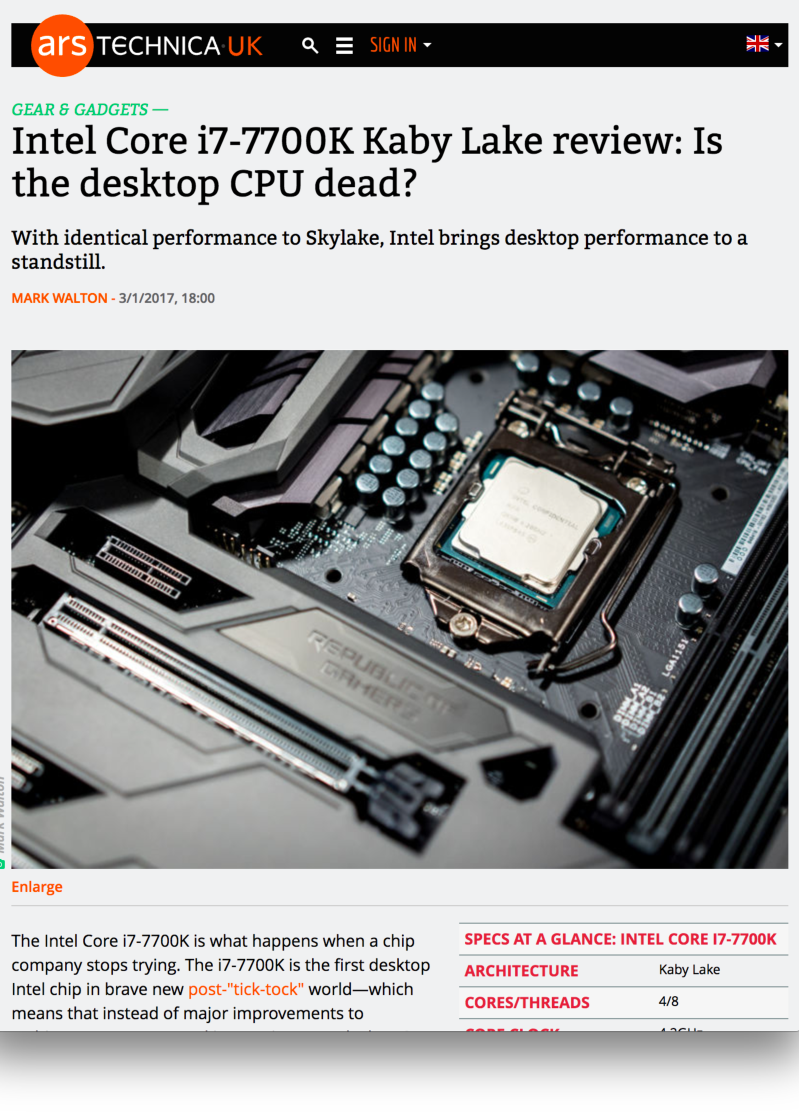
\includegraphics[width=\textwidth]{news.pdf}
\end{frame}

\begin{frame}[noframenumbering,plain]{arsTECHNICA UK - 03.01.2017 (2)}
  „With low-power laptops and all-in-ones continuing to outsell desktops—and with high-end workloads like video editing, 3D animation, and machine learning increasingly being offloaded to GPUs -- perhaps it was inevitable that Intel would stop caring so much about its high-end consumer CPUs.“
\end{frame}
\maketitle

\section*{Gliederung}
\begin{frame}[noframenumbering,plain]{Gliederung}
  \tableofcontents[hideallsubsections]
\end{frame}

\section{Nebenläufigkeit / Parallelisierung}
  \begin{frame}{Parallel}
  \setcounter{framenumber}{1}
    \begin{columns}[c]
    \column{.5\textwidth}
      \begin{itemize}
        \item Synonyme: \textit{nebeneinander, nebenläufig}
        \item Informatik:\\parallel ≠ nebenläufig!
        \item „schneller als sequenzielles Programm, durch gleichzeitiges Ausführen von \alert{Anweisungen}“
        \item Multi-Processing
      \end{itemize}
    \column{.5\textwidth}
    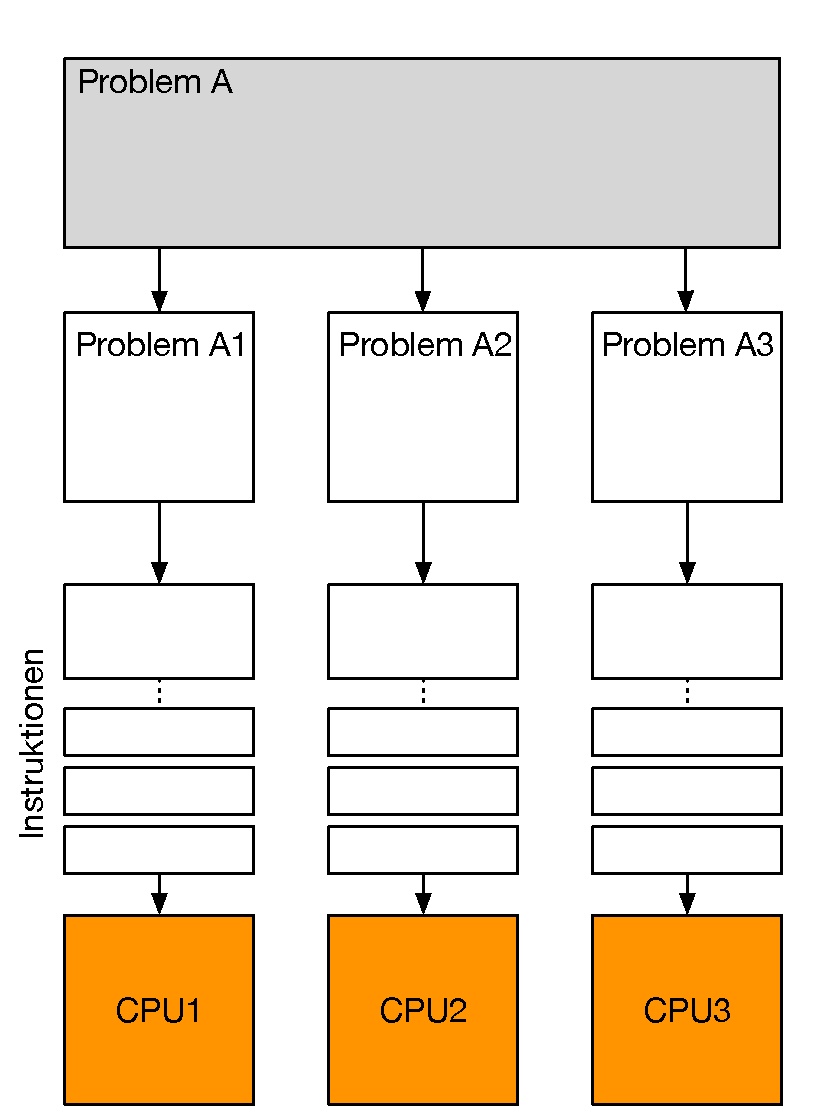
\includegraphics[width=\textwidth]{parallel.pdf}
    \end{columns}
  \end{frame}

  \note[itemize]{
      \item deutscher Begriff schwierig
      \item Aufteilen des Problems in Teilprobleme
      \item Teile können, müssen aber nicht zusammengehörend sein
  }

  \begin{frame}{Nebenläufig}
    \begin{columns}[c]
    \column{.5\textwidth}
      \begin{itemize}
        \item concurrent (engl.)
        \item „Systeme, welche zur gleichen Zeit mehrere \alert{Aufgaben} haben“
        \item muss nicht zwangsläufig parallel sein
        \item Multi-Tasking
      \end{itemize}
    \column{.5\textwidth}
      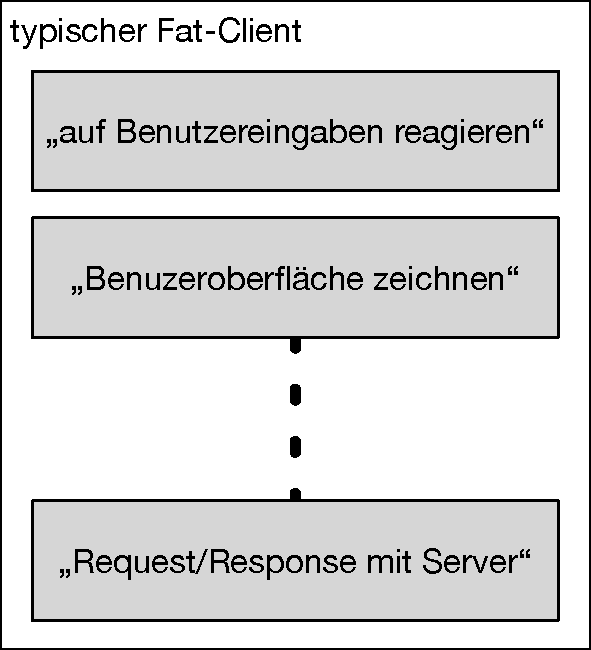
\includegraphics[width=\textwidth]{concurrent.pdf}
    \end{columns}
  \end{frame}

  \note[itemize]{}

  \begin{frame}{Rob Pike - „Concurrency Is Not Parallelism“ (1)}
    \begin{itemize}
      \item „Concurrency is about dealing with lots of things at once.“
      \item „Parallelism is about doing lots of things at once.“
      \item „Concurrency is about structure, parallelism is about execution.“
    \end{itemize}
  \end{frame}

  \note[itemize]{
      \item Google, Go-Lang
      \item interessanter Talk auf Youtube
  }

  \begin{frame}{Rob Pike - „Concurrency Is Not Parallelism“ (2)}
    
\includegraphics[width=\textwidth]{gophersimple1.pdf}
    \begin{itemize}
      \item sequenziell
    \end{itemize}
  \end{frame}

  \begin{frame}{Rob Pike - „Concurrency Is Not Parallelism“ (3)}
    
\includegraphics[width=\textwidth]{gophersimple3.pdf}
    \begin{itemize}
      \item mehrere Cores, jedoch keine Optimierung
    \end{itemize}
  \end{frame}

  \begin{frame}{Rob Pike - „Concurrency Is Not Parallelism“ (4)}
    
\includegraphics[width=\textwidth]{gophersimple2.pdf}
    \begin{itemize}
      \item parallel
    \end{itemize}
  \end{frame}

  \begin{frame}{Rob Pike - „Concurrency Is Not Parallelism“ (5)}
    
\includegraphics[width=\textwidth]{gophercomplex0.pdf}
    \begin{itemize}
      \item concurrent
    \end{itemize}
  \end{frame}

% \section{Threads / Locking}
%   \begin{frame}{Was ist ein Thread?}
%     \begin{columns}[c]
%     \column{.5\textwidth}
%       \begin{itemize}
%         \item Shared Memory
%       \end{itemize}
%     \column{.5\textwidth}
%       \begin{figure}
%         \centering
%         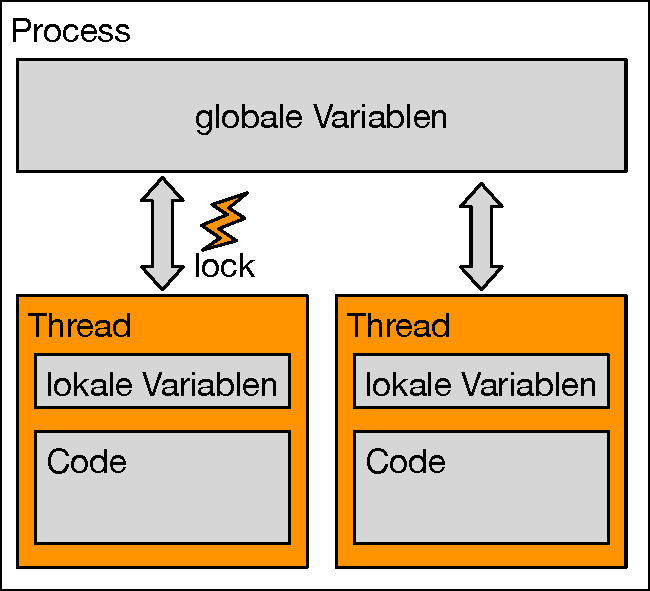
\includegraphics[width=\textwidth]{threads.pdf}
%       \end{figure}
%     \end{columns}
%   \end{frame}
%
%   \begin{frame}{Was ist ein Lock?}
%     \begin{columns}[c]
%     \column{.5\textwidth}
%       \begin{itemize}
%       \item{Dining philosophers problem}
%       \end{itemize}
%     \column{.5\textwidth}
%       \begin{figure}
%         \centering
%         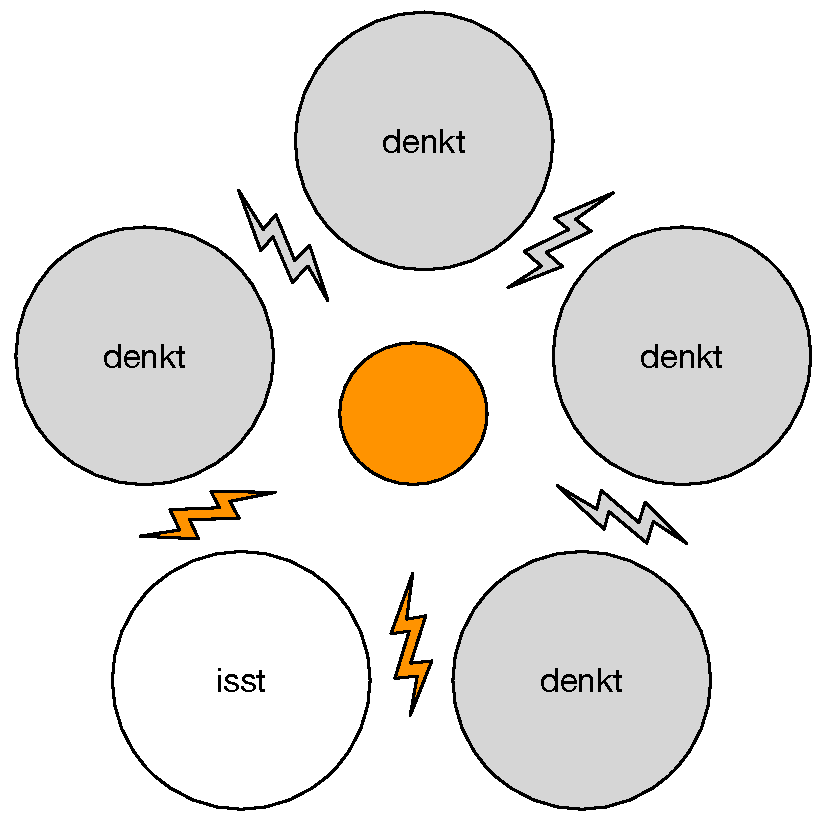
\includegraphics[width=\textwidth]{philosophers_table.pdf}
%       \end{figure}
%     \end{columns}
%   \end{frame}
%
%   \begin{frame}{Häufige Bugs}
%     \begin{columns}[c]
%     \column{.5\textwidth}
%       \textbf{Race-Condition}
%       \begin{itemize}
%         \item ++
%         \item ++
%       \end{itemize}
%     \column{.5\textwidth}
%       \textbf{Deadlock}
%       \begin{itemize}
%         \item --
%         \item --
%       \end{itemize}
%     \end{columns}
%   \end{frame}
%
%   \begin{frame}{Fazit: Threads Programming}
%     \begin{itemize}
%       \item „State is Evil“
%     \end{itemize}
%   \end{frame}
%
%   \note[itemize]{
%       \item Viele Sprachen besitzen threads als feature,
%       \item wenige Sprachen helfen mit Tooling oder Abstraktion dem Programmierer selbst!
%   }

\section{Functional Paradigm 101}
  \begin{frame}{Functional Paradigm 101}
    \begin{itemize}
      \item reine Funktionale Sprachen
      \item imutable // mutable
      \item no side-effects
      \item deterministic
      \item data-in <-> data-out
      \item functions as first-class citizens
      \item lamdas
    \end{itemize}
  \end{frame}

\section{Elixir}
  \begin{frame}{Elixir}
    \begin{itemize}
      \item moderne Variante von Erlang (1987, Ericsson)
      \item Beam-VM
      \item Fault-Taulerant
      \item „Let it crash“
      \item Supervision-Trees
      \item Shared \& Distributed Memory
      \item Open Telecom Platform (OTP)
    \end{itemize}
  \end{frame}

  \begin{frame}{OTP / Actor-Model}
    \begin{columns}[c]
    \column{.5\textwidth}
    \begin{itemize}
      \item unabhängige Akteure
      \item Message-Passing
      \item FIFO-Verhalten von \alert{Mailboxes}
      \item Locks werden nicht gebraucht
      \item Alternativen:
        \begin{itemize}
          \item Akka (Java/Scala)
          \item Akka.NET
          \item Pykka (Python)
          \item CAF (C++)
          \item Celluloid (Ruby)
        \end{itemize}
    \end{itemize}
    \column{.5\textwidth}
      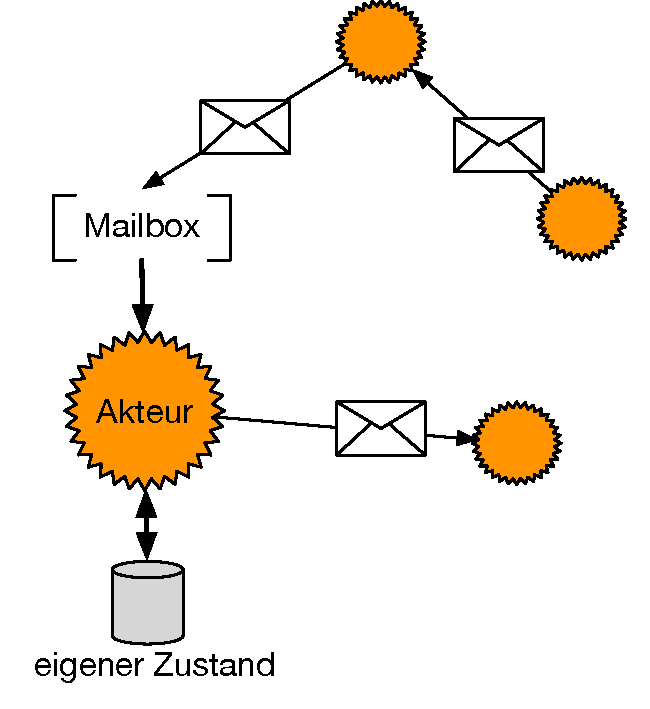
\includegraphics[width=\textwidth]{actors.pdf}
    \end{columns}
  \end{frame}

  \begin{frame}{List-Processing in Elixir: map (1)}
    \begin{columns}[c]
    \column{.5\textwidth}
      \begin{itemize}
        \item Traversieren der Elemente
        \item Nutzen von transform-function
        \item Ergebnis von gleichem oder verschiedenen Collection-Typ
      \end{itemize}
    \column{.5\textwidth}
    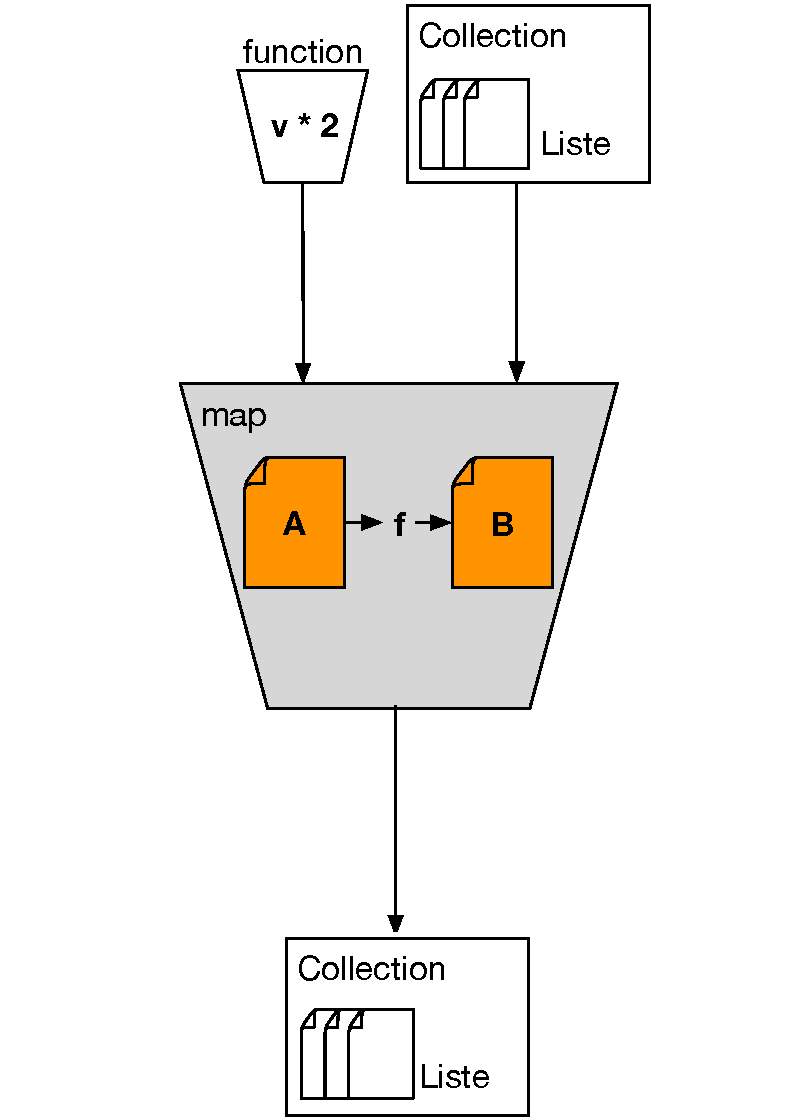
\includegraphics[width=\textwidth]{map.pdf}
    \end{columns}
  \end{frame}

  \begin{frame}{List-Processing in Elixir: map (2)}
    \begin{itemize}[<+->]
    \item
      \texttt{iex> Enum.map [1, 2, 3], fn x -> x + 1 end} \\
      \textbf{[2, 3, 4]} \\
    \item
      \texttt{iex> Enum.map [1, 2, 3], \&(\&1 * \&1)} \\
      \textbf{[1, 4, 9]} \\
    \item
      \texttt{iex> defmodule Math do \\
            ...> def multWithKey(\{k, v\}), do: k * v \\
            ...> end\\
      }
      \textbf{...} \\
      \texttt{iex> list = Enum.with\_index([1, 2, 3])} \\
      \textbf{[\{1, 0\}, \{2, 1\}, \{3, 2\}]} \\
      \texttt{iex> Enum.map list, \&Math.multWithKey/1} \\
      \textbf{[0, 2, 6]} \\
    \end{itemize}
  \end{frame}

  \begin{frame}{List-Processing in Elixir: reduce (1)}
    \begin{columns}[c]
    \column{.5\textwidth}
      \begin{itemize}
        \item Traversieren der Elemente
        \item Nutzen von aggregate-function und Startwert
        \item Mitführen von accumulator
        \item „Reduzieren“ der Elemente auf einzelnen gemeinsamen Wert
        \item auch \texttt{foldr, foldl} genannt
      \end{itemize}
    \column{.5\textwidth}
    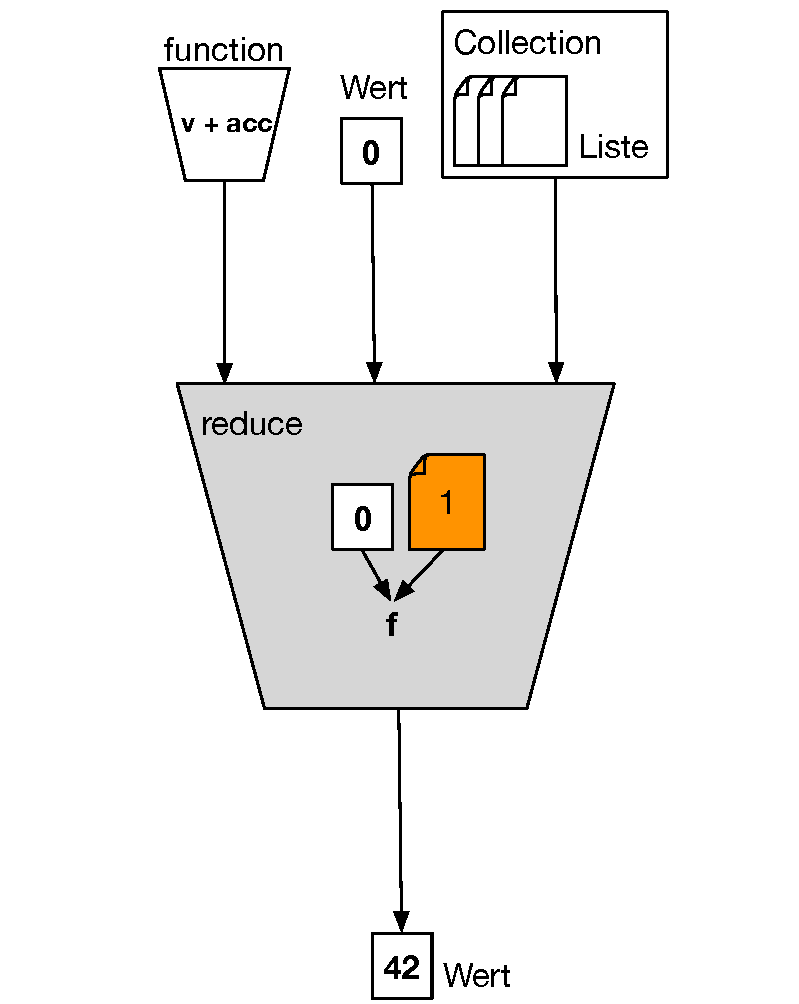
\includegraphics[width=\textwidth]{reduce.pdf}
    \end{columns}
  \end{frame}

  \begin{frame}{List-Processing in Elixir: reduce (2)}
    \begin{itemize}[<+->]
      \item \texttt{iex> List.foldl [1, 2, 3, 4], 0, \&(\&1 + \&2)} \\
            \textbf{10}
    \end{itemize}
  \end{frame}

  \begin{frame}{List-Processing in Elixir: filter (1)}
    \begin{columns}[c]
    \column{.5\textwidth}
      \begin{itemize}
        \item Traversieren der Elemente
        \item Nutzen von predicate-function
        \item Teilmenge bilden, welche Elemente enthält, welche Anforderung erfüllen
      \end{itemize}
    \column{.5\textwidth}
    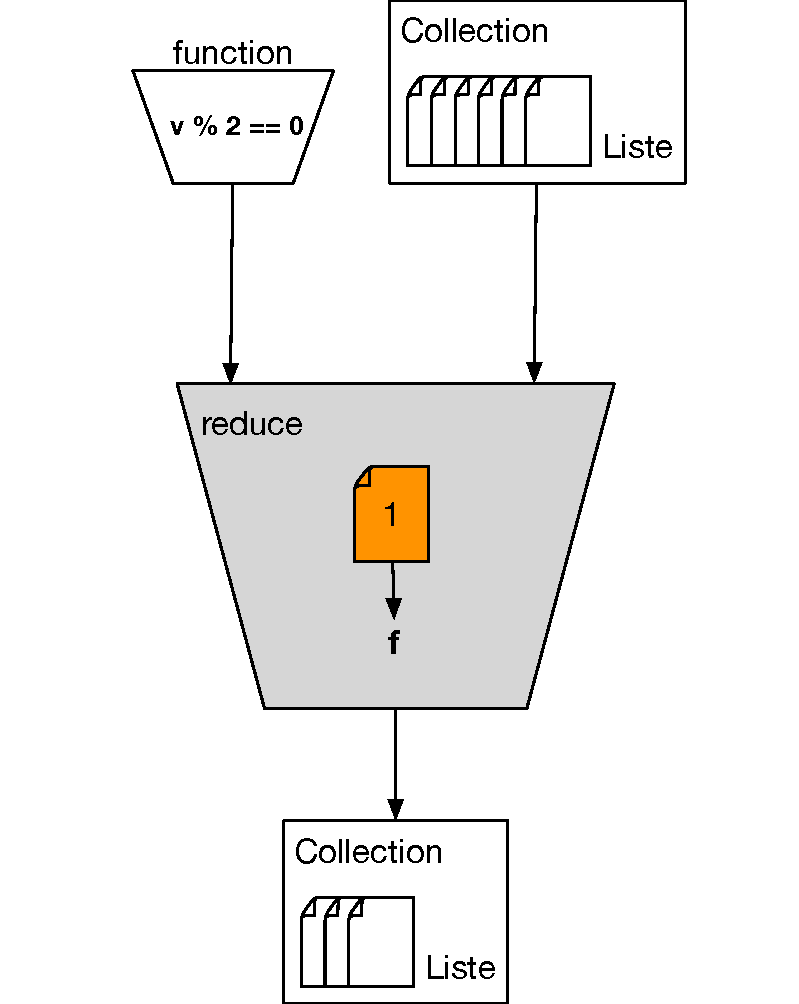
\includegraphics[width=\textwidth]{filter.pdf}
    \end{columns}
  \end{frame}

  \begin{frame}{List-Processing in Elixir: filter (2)}
  \end{frame}

  \begin{frame}{Elixir-Streams}
  \end{frame}

\section{Fazit}
  \begin{frame}{Fazit: Functional Programming}
    \begin{columns}[c]
    \column{.5\textwidth}
      \textbf{Vorteile}
      \begin{itemize}
        \item composeability of behaviors
        \item Art und Abfolge der Anweisung kann genau und deklarativ bestimmt werden
      \end{itemize}
    \column{.5\textwidth}
      \textbf{Nachteile}
      \begin{itemize}
        \item Punkt 1
        \item Punkt 2
      \end{itemize}
    \end{columns}
  \end{frame}

  \begin{frame}{Functional Style in Imperative Languages}
  \end{frame}
\end{document}
